\documentclass{article}\usepackage[]{graphicx}\usepackage[]{xcolor}
% maxwidth is the original width if it is less than linewidth
% otherwise use linewidth (to make sure the graphics do not exceed the margin)
\makeatletter
\def\maxwidth{ %
  \ifdim\Gin@nat@width>\linewidth
    \linewidth
  \else
    \Gin@nat@width
  \fi
}
\makeatother

\definecolor{fgcolor}{rgb}{0.345, 0.345, 0.345}
\newcommand{\hlnum}[1]{\textcolor[rgb]{0.686,0.059,0.569}{#1}}%
\newcommand{\hlstr}[1]{\textcolor[rgb]{0.192,0.494,0.8}{#1}}%
\newcommand{\hlcom}[1]{\textcolor[rgb]{0.678,0.584,0.686}{\textit{#1}}}%
\newcommand{\hlopt}[1]{\textcolor[rgb]{0,0,0}{#1}}%
\newcommand{\hlstd}[1]{\textcolor[rgb]{0.345,0.345,0.345}{#1}}%
\newcommand{\hlkwa}[1]{\textcolor[rgb]{0.161,0.373,0.58}{\textbf{#1}}}%
\newcommand{\hlkwb}[1]{\textcolor[rgb]{0.69,0.353,0.396}{#1}}%
\newcommand{\hlkwc}[1]{\textcolor[rgb]{0.333,0.667,0.333}{#1}}%
\newcommand{\hlkwd}[1]{\textcolor[rgb]{0.737,0.353,0.396}{\textbf{#1}}}%
\let\hlipl\hlkwb

\usepackage{framed}
\makeatletter
\newenvironment{kframe}{%
 \def\at@end@of@kframe{}%
 \ifinner\ifhmode%
  \def\at@end@of@kframe{\end{minipage}}%
  \begin{minipage}{\columnwidth}%
 \fi\fi%
 \def\FrameCommand##1{\hskip\@totalleftmargin \hskip-\fboxsep
 \colorbox{shadecolor}{##1}\hskip-\fboxsep
     % There is no \\@totalrightmargin, so:
     \hskip-\linewidth \hskip-\@totalleftmargin \hskip\columnwidth}%
 \MakeFramed {\advance\hsize-\width
   \@totalleftmargin\z@ \linewidth\hsize
   \@setminipage}}%
 {\par\unskip\endMakeFramed%
 \at@end@of@kframe}
\makeatother

\definecolor{shadecolor}{rgb}{.97, .97, .97}
\definecolor{messagecolor}{rgb}{0, 0, 0}
\definecolor{warningcolor}{rgb}{1, 0, 1}
\definecolor{errorcolor}{rgb}{1, 0, 0}
\newenvironment{knitrout}{}{} % an empty environment to be redefined in TeX

\usepackage{alltt}
\usepackage[sc]{mathpazo}
\renewcommand{\sfdefault}{lmss}
\renewcommand{\ttdefault}{lmtt}
\usepackage[T1]{fontenc}
\usepackage{geometry}
\geometry{verbose,tmargin=2.5cm,bmargin=2.5cm,lmargin=2.5cm,rmargin=2.5cm}
\setcounter{secnumdepth}{2}
\setcounter{tocdepth}{2}
\usepackage[unicode=true,pdfusetitle,
 bookmarks=true,bookmarksnumbered=true,bookmarksopen=true,bookmarksopenlevel=2,
 breaklinks=false,pdfborder={0 0 1},backref=false,colorlinks=false]
 {hyperref}
\hypersetup{
 pdfstartview={XYZ null null 1}}

\makeatletter
%%%%%%%%%%%%%%%%%%%%%%%%%%%%%% User specified LaTeX commands.
\renewcommand{\textfraction}{0.05}
\renewcommand{\topfraction}{0.8}
\renewcommand{\bottomfraction}{0.8}
\renewcommand{\floatpagefraction}{0.75}

\makeatother
\IfFileExists{upquote.sty}{\usepackage{upquote}}{}
\begin{document}



\title{\title{\title{\title{\title{\title{\title{\title{}}}}}}}}



\maketitle
The results below are generated from an R script.

\begin{knitrout}
\definecolor{shadecolor}{rgb}{0.969, 0.969, 0.969}\color{fgcolor}\begin{kframe}
\begin{alltt}
\hlcom{# Liberías necesarias para resolver el ejercicio}
\hlkwd{library}\hlstd{(liver)}
\end{alltt}


{\ttfamily\noindent\itshape\color{messagecolor}{\#\# \\\#\# Attaching package: 'liver'}}

{\ttfamily\noindent\itshape\color{messagecolor}{\#\# The following object is masked from 'package:base':\\\#\# \\\#\# \ \ \ \ transform}}\begin{alltt}
\hlkwd{library}\hlstd{(caret)}
\hlkwd{library}\hlstd{(caTools)}
\hlkwd{library}\hlstd{(rpart.plot)}

\hlcom{# Datos}
\hlkwd{data}\hlstd{(adult)}

\hlcom{# Resumen}
\hlkwd{summary}\hlstd{(adult)}
\end{alltt}
\begin{verbatim}
##       age              workclass      demogweight             education    
##  Min.   :17.0   ?           : 2794   Min.   :  12285   HS-grad     :15750  
##  1st Qu.:28.0   Gov         : 6536   1st Qu.: 117550   Some-college:10860  
##  Median :37.0   Never-worked:   10   Median : 178215   Bachelors   : 7962  
##  Mean   :38.6   Private     :33780   Mean   : 189685   Masters     : 2627  
##  3rd Qu.:48.0   Self-emp    : 5457   3rd Qu.: 237713   Assoc-voc   : 2058  
##  Max.   :90.0   Without-pay :   21   Max.   :1490400   11th        : 1812  
##                                                        (Other)     : 7529  
##  education.num         marital.status            occupation            relationship  
##  Min.   : 1.00   Divorced     : 6613   Craft-repair   : 6096   Husband       :19537  
##  1st Qu.: 9.00   Married      :22847   Prof-specialty : 6071   Not-in-family :12546  
##  Median :10.00   Never-married:16096   Exec-managerial: 6019   Other-relative: 1506  
##  Mean   :10.06   Separated    : 1526   Adm-clerical   : 5603   Own-child     : 7577  
##  3rd Qu.:12.00   Widowed      : 1516   Sales          : 5470   Unmarried     : 5118  
##  Max.   :16.00                         Other-service  : 4920   Wife          : 2314  
##                                        (Other)        :14419                         
##                  race          gender       capital.gain      capital.loss    
##  Amer-Indian-Eskimo:  470   Female:16156   Min.   :    0.0   Min.   :   0.00  
##  Asian-Pac-Islander: 1504   Male  :32442   1st Qu.:    0.0   1st Qu.:   0.00  
##  Black             : 4675                  Median :    0.0   Median :   0.00  
##  Other             :  403                  Mean   :  582.4   Mean   :  87.94  
##  White             :41546                  3rd Qu.:    0.0   3rd Qu.:   0.00  
##                                            Max.   :41310.0   Max.   :4356.00  
##                                                                               
##  hours.per.week        native.country    income     
##  Min.   : 1.00   United-States:43613   <=50K:37155  
##  1st Qu.:40.00   Mexico       :  949   >50K :11443  
##  Median :40.00   ?            :  847                
##  Mean   :40.37   Philippines  :  292                
##  3rd Qu.:45.00   Germany      :  206                
##  Max.   :99.00   Puerto-Rico  :  184                
##                  (Other)      : 2507
\end{verbatim}
\begin{alltt}
\hlcom{# Partición de los datos }

\hlcom{# Mediante una semilla conseguimos que el ejercicio sea reproducible}
\hlkwd{set.seed}\hlstd{(}\hlnum{12321}\hlstd{)}

\hlcom{# Usamos el 20% de la base de datos como conjunto de entrenamiento y el resto como conjunto de validación}
\hlstd{sample} \hlkwb{=} \hlkwd{sample.split}\hlstd{(adult}\hlopt{$}\hlstd{income,} \hlkwc{SplitRatio}\hlstd{=}\hlnum{0.2}\hlstd{)}
\hlstd{datos.train}  \hlkwb{=} \hlkwd{subset}\hlstd{(adult, sample}\hlopt{==}\hlnum{TRUE}\hlstd{)}
\hlstd{datos.valid}   \hlkwb{=} \hlkwd{subset}\hlstd{(adult, sample}\hlopt{==}\hlnum{FALSE}\hlstd{)}

\hlcom{# Entrenamos un modelo sobre la muestra de entrenamiento empleando todas las variables}

\hlstd{traindata} \hlkwb{=} \hlstd{datos.train[,}\hlopt{-}\hlnum{15}\hlstd{]}
\hlstd{trainclasses} \hlkwb{=} \hlstd{datos.train[,}\hlnum{15}\hlstd{]}
\hlstd{validdata} \hlkwb{=} \hlstd{datos.valid[,}\hlopt{-}\hlnum{15}\hlstd{]}
\hlstd{validclasses} \hlkwb{=} \hlstd{datos.valid[,}\hlnum{15}\hlstd{]}

\hlstd{ctrl} \hlkwb{<-} \hlkwd{trainControl}\hlstd{(}\hlkwc{method} \hlstd{=} \hlstr{"cv"}\hlstd{,} \hlkwc{number} \hlstd{=} \hlnum{5}\hlstd{)}

\hlcom{# Entrenamos un knn }

\hlcom{# Entrenamos un knn en cada una de las particiones}
\hlstd{ctrl} \hlkwb{<-} \hlkwd{trainControl}\hlstd{(}\hlkwc{method} \hlstd{=} \hlstr{"cv"}\hlstd{,} \hlkwc{number} \hlstd{=} \hlnum{5}\hlstd{)}
\hlstd{traindata1} \hlkwb{=} \hlkwd{as.data.frame}\hlstd{(}\hlkwd{cbind}\hlstd{(traindata}\hlopt{$}\hlstd{age,traindata}\hlopt{$}\hlstd{hours.per.week))}
\hlstd{knn.fit1} \hlkwb{=} \hlkwd{train}\hlstd{(traindata1,trainclasses,}\hlkwc{method}\hlstd{=}\hlstr{"knn"}\hlstd{,}\hlkwc{trControl}\hlstd{=ctrl,} \hlkwc{preProcess} \hlstd{=} \hlkwd{c}\hlstd{(}\hlstr{"center"}\hlstd{,}\hlstr{"scale"}\hlstd{))}
\hlstd{knn.fit1}
\end{alltt}
\begin{verbatim}
## k-Nearest Neighbors 
## 
## 9720 samples
##    2 predictor
##    2 classes: '<=50K', '>50K' 
## 
## Pre-processing: centered (2), scaled (2) 
## Resampling: Cross-Validated (5 fold) 
## Summary of sample sizes: 7776, 7776, 7775, 7777, 7776 
## Resampling results across tuning parameters:
## 
##   k  Accuracy   Kappa    
##   5  0.7562751  0.1631052
##   7  0.7609056  0.1704753
##   9  0.7644034  0.1784621
## 
## Accuracy was used to select the optimal model using the largest value.
## The final value used for the model was k = 9.
\end{verbatim}
\begin{alltt}
\hlcom{# Modelo Final}
\hlstd{knn.fit1}\hlopt{$}\hlstd{finalModel}
\end{alltt}
\begin{verbatim}
## 9-nearest neighbor model
## Training set outcome distribution:
## 
## <=50K  >50K 
##  7431  2289
\end{verbatim}
\begin{alltt}
\hlcom{# Resultados del modelo para cada una de las submuestras}
\hlstd{knn.fit1}\hlopt{$}\hlstd{resample}
\end{alltt}
\begin{verbatim}
##    Accuracy     Kappa Resample
## 1 0.7664609 0.2006926    Fold1
## 2 0.7637674 0.1657707    Fold4
## 3 0.7629820 0.1784940    Fold3
## 4 0.7613169 0.1660047    Fold2
## 5 0.7674897 0.1813486    Fold5
\end{verbatim}
\begin{alltt}
\hlcom{# Error de clasificación en train}
\hlcom{# sobre la partición de entrenamiento}
\hlstd{prediction} \hlkwb{=} \hlkwd{predict}\hlstd{(knn.fit1}\hlopt{$}\hlstd{finalModel, traindata1,} \hlkwc{type} \hlstd{=} \hlstr{'class'}\hlstd{)}
\hlstd{cf} \hlkwb{=} \hlkwd{confusionMatrix}\hlstd{(prediction,} \hlkwd{as.factor}\hlstd{(trainclasses),}\hlkwc{positive}\hlstd{=}\hlstr{">50K"}\hlstd{)}
\hlkwd{print}\hlstd{(cf)}
\end{alltt}
\begin{verbatim}
## Confusion Matrix and Statistics
## 
##           Reference
## Prediction <=50K >50K
##      <=50K  7412 2287
##      >50K     19    2
##                                           
##                Accuracy : 0.7628          
##                  95% CI : (0.7542, 0.7712)
##     No Information Rate : 0.7645          
##     P-Value [Acc > NIR] : 0.6628          
##                                           
##                   Kappa : -0.0026         
##                                           
##  Mcnemar's Test P-Value : <2e-16          
##                                           
##             Sensitivity : 0.0008737       
##             Specificity : 0.9974431       
##          Pos Pred Value : 0.0952381       
##          Neg Pred Value : 0.7642025       
##              Prevalence : 0.2354938       
##          Detection Rate : 0.0002058       
##    Detection Prevalence : 0.0021605       
##       Balanced Accuracy : 0.4991584       
##                                           
##        'Positive' Class : >50K            
## 
\end{verbatim}
\begin{alltt}
\hlcom{# Entrenamos un árbol en cada una de las particiones}
\hlstd{dt.fit1} \hlkwb{=} \hlkwd{train}\hlstd{(traindata,trainclasses,}\hlkwc{method}\hlstd{=}\hlstr{"rpart"}\hlstd{,}\hlkwc{trControl}\hlstd{=ctrl)}
\hlstd{dt.fit1}
\end{alltt}
\begin{verbatim}
## CART 
## 
## 9720 samples
##   14 predictor
##    2 classes: '<=50K', '>50K' 
## 
## No pre-processing
## Resampling: Cross-Validated (5 fold) 
## Summary of sample sizes: 7775, 7776, 7777, 7776, 7776 
## Resampling results across tuning parameters:
## 
##   cp          Accuracy   Kappa    
##   0.03363914  0.8299390  0.4903102
##   0.04062910  0.8180055  0.4657887
##   0.10943644  0.7926955  0.2528124
## 
## Accuracy was used to select the optimal model using the largest value.
## The final value used for the model was cp = 0.03363914.
\end{verbatim}
\begin{alltt}
\hlcom{# Modelo Final}
\hlstd{dt.fit1}\hlopt{$}\hlstd{finalModel}
\end{alltt}
\begin{verbatim}
## n= 9720 
## 
## node), split, n, loss, yval, (yprob)
##       * denotes terminal node
## 
##  1) root 9720 2289 <=50K (0.76450617 0.23549383)  
##    2) relationship=Not-in-family,Other-relative,Own-child,Unmarried 5315  335 <=50K (0.93697084 0.06302916) *
##    3) relationship=Husband,Wife 4405 1954 <=50K (0.55641317 0.44358683)  
##      6) occupation=?,Adm-clerical,Craft-repair,Farming-fishing,Handlers-cleaners,Machine-op-inspct,Other-service,Priv-house-serv,Transport-moving 2336  669 <=50K (0.71361301 0.28638699)  
##       12) capital.gain< 5095.5 2239  574 <=50K (0.74363555 0.25636445) *
##       13) capital.gain>=5095.5 97    2 >50K (0.02061856 0.97938144) *
##      7) occupation=Armed-Forces,Exec-managerial,Prof-specialty,Protective-serv,Sales,Tech-support 2069  784 >50K (0.37892702 0.62107298) *
\end{verbatim}
\begin{alltt}
\hlkwd{rpart.plot}\hlstd{(dt.fit1}\hlopt{$}\hlstd{finalModel)}
\end{alltt}
\end{kframe}

{\centering 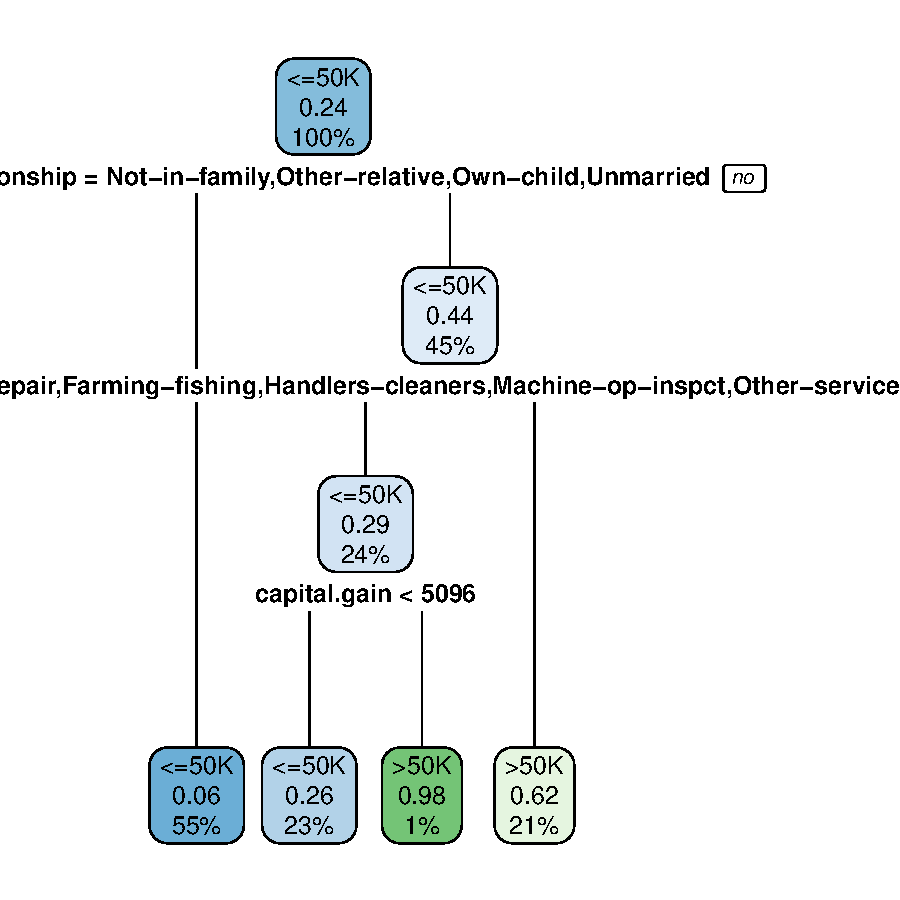
\includegraphics[width=.6\linewidth]{figure/EVAL1-SOLUCION-Rnwauto-report-1} 

}


\begin{kframe}\begin{alltt}
\hlcom{# Resultados del modelo para cada una de las submuestras}
\hlstd{dt.fit1}\hlopt{$}\hlstd{resample}
\end{alltt}
\begin{verbatim}
##    Accuracy     Kappa Resample
## 1 0.8313625 0.4635475    Fold1
## 2 0.8179012 0.4393843    Fold2
## 3 0.8353909 0.4999293    Fold5
## 4 0.8266461 0.5040981    Fold4
## 5 0.8383942 0.5445919    Fold3
\end{verbatim}
\begin{alltt}
\hlcom{# Error de clasificación en train}
\hlcom{# sobre la partición de entrenamiento}
\hlstd{prediction} \hlkwb{=} \hlkwd{predict}\hlstd{(dt.fit1}\hlopt{$}\hlstd{finalModel, datos.train,} \hlkwc{type} \hlstd{=} \hlstr{'class'}\hlstd{)}
\hlstd{cf} \hlkwb{=} \hlkwd{confusionMatrix}\hlstd{(prediction,} \hlkwd{as.factor}\hlstd{(trainclasses),}\hlkwc{positive}\hlstd{=}\hlstr{">50K"}\hlstd{)}
\hlkwd{print}\hlstd{(cf)}
\end{alltt}
\begin{verbatim}
## Confusion Matrix and Statistics
## 
##           Reference
## Prediction <=50K >50K
##      <=50K  6645  909
##      >50K    786 1380
##                                           
##                Accuracy : 0.8256          
##                  95% CI : (0.8179, 0.8331)
##     No Information Rate : 0.7645          
##     P-Value [Acc > NIR] : < 2.2e-16       
##                                           
##                   Kappa : 0.5065          
##                                           
##  Mcnemar's Test P-Value : 0.003044        
##                                           
##             Sensitivity : 0.6029          
##             Specificity : 0.8942          
##          Pos Pred Value : 0.6371          
##          Neg Pred Value : 0.8797          
##              Prevalence : 0.2355          
##          Detection Rate : 0.1420          
##    Detection Prevalence : 0.2228          
##       Balanced Accuracy : 0.7486          
##                                           
##        'Positive' Class : >50K            
## 
\end{verbatim}
\begin{alltt}
\hlcom{# sobre la partición de validación}
\hlstd{prediction} \hlkwb{=} \hlkwd{predict}\hlstd{(dt.fit1}\hlopt{$}\hlstd{finalModel, datos.valid,} \hlkwc{type} \hlstd{=} \hlstr{'class'}\hlstd{)}
\hlstd{cf} \hlkwb{=} \hlkwd{confusionMatrix}\hlstd{(prediction,} \hlkwd{as.factor}\hlstd{(validclasses),}\hlkwc{positive}\hlstd{=}\hlstr{">50K"}\hlstd{)}
\hlkwd{print}\hlstd{(cf)}
\end{alltt}
\begin{verbatim}
## Confusion Matrix and Statistics
## 
##           Reference
## Prediction <=50K  >50K
##      <=50K 26700  3662
##      >50K   3024  5492
##                                           
##                Accuracy : 0.828           
##                  95% CI : (0.8242, 0.8318)
##     No Information Rate : 0.7645          
##     P-Value [Acc > NIR] : < 2.2e-16       
##                                           
##                   Kappa : 0.5105          
##                                           
##  Mcnemar's Test P-Value : 6.683e-15       
##                                           
##             Sensitivity : 0.6000          
##             Specificity : 0.8983          
##          Pos Pred Value : 0.6449          
##          Neg Pred Value : 0.8794          
##              Prevalence : 0.2355          
##          Detection Rate : 0.1413          
##    Detection Prevalence : 0.2190          
##       Balanced Accuracy : 0.7491          
##                                           
##        'Positive' Class : >50K            
## 
\end{verbatim}
\end{kframe}
\end{knitrout}

The R session information (including the OS info, R version and all
packages used):

\begin{knitrout}
\definecolor{shadecolor}{rgb}{0.969, 0.969, 0.969}\color{fgcolor}\begin{kframe}
\begin{alltt}
\hlkwd{sessionInfo}\hlstd{()}
\end{alltt}
\begin{verbatim}
## R version 4.3.1 (2023-06-16)
## Platform: x86_64-pc-linux-gnu (64-bit)
## Running under: Ubuntu 20.04.6 LTS
## 
## Matrix products: default
## BLAS:   /usr/lib/x86_64-linux-gnu/atlas/libblas.so.3.10.3 
## LAPACK: /usr/lib/x86_64-linux-gnu/atlas/liblapack.so.3.10.3;  LAPACK version 3.9.0
## 
## locale:
##  [1] LC_CTYPE=es_ES.UTF-8       LC_NUMERIC=C               LC_TIME=es_ES.UTF-8       
##  [4] LC_COLLATE=es_ES.UTF-8     LC_MONETARY=es_ES.UTF-8    LC_MESSAGES=es_ES.UTF-8   
##  [7] LC_PAPER=es_ES.UTF-8       LC_NAME=C                  LC_ADDRESS=C              
## [10] LC_TELEPHONE=C             LC_MEASUREMENT=es_ES.UTF-8 LC_IDENTIFICATION=C       
## 
## time zone: Europe/Madrid
## tzcode source: system (glibc)
## 
## attached base packages:
## [1] stats     graphics  grDevices utils     datasets  methods   base     
## 
## other attached packages:
##  [1] liver_1.15       ggfortify_0.4.16 factoextra_1.0.7 mlbench_2.1-3.1  readxl_1.4.3    
##  [6] caret_6.0-94     lattice_0.21-9   ggplot2_3.4.3    rpart.plot_3.1.1 rpart_4.1.19    
## [11] caTools_1.18.2   dplyr_1.1.3      ISLR2_1.3-2     
## 
## loaded via a namespace (and not attached):
##  [1] tidyselect_1.2.0     timeDate_4022.108    farver_2.1.1         bitops_1.0-7        
##  [5] fastmap_1.1.1        pROC_1.18.4          digest_0.6.33        timechange_0.2.0    
##  [9] lifecycle_1.0.3      survival_3.5-7       magrittr_2.0.3       compiler_4.3.1      
## [13] rlang_1.1.1          tools_4.3.1          utf8_1.2.3           yaml_2.3.7          
## [17] data.table_1.14.8    knitr_1.44           labeling_0.4.3       plyr_1.8.9          
## [21] withr_2.5.1          purrr_1.0.2          nnet_7.3-19          grid_4.3.1          
## [25] stats4_4.3.1         fansi_1.0.5          e1071_1.7-13         colorspace_2.1-0    
## [29] future_1.33.0        globals_0.16.2       scales_1.2.1         iterators_1.0.14    
## [33] MASS_7.3-60          tinytex_0.47         cli_3.6.1            rmarkdown_2.25      
## [37] generics_0.1.3       rstudioapi_0.15.0    future.apply_1.11.0  reshape2_1.4.4      
## [41] tzdb_0.4.0           proxy_0.4-27         stringr_1.5.0        splines_4.3.1       
## [45] parallel_4.3.1       cellranger_1.1.0     vctrs_0.6.3          hardhat_1.3.0       
## [49] Matrix_1.6-1.1       hms_1.1.3            ggrepel_0.9.3        listenv_0.9.0       
## [53] foreach_1.5.2        tidyr_1.3.0          gower_1.0.1          recipes_1.0.8       
## [57] glue_1.6.2           parallelly_1.36.0    codetools_0.2-19     lubridate_1.9.3     
## [61] stringi_1.7.12       gtable_0.3.4         munsell_0.5.0        tibble_3.2.1        
## [65] pillar_1.9.0         htmltools_0.5.6.1    ipred_0.9-14         lava_1.7.2.1        
## [69] R6_2.5.1             evaluate_0.22        readr_2.1.4          highr_0.10          
## [73] class_7.3-22         Rcpp_1.0.11          gridExtra_2.3        nlme_3.1-163        
## [77] prodlim_2023.08.28   xfun_0.40            pkgconfig_2.0.3      ModelMetrics_1.2.2.2
\end{verbatim}
\begin{alltt}
\hlkwd{Sys.time}\hlstd{()}
\end{alltt}
\begin{verbatim}
## [1] "2023-11-02 17:28:54 CET"
\end{verbatim}
\end{kframe}
\end{knitrout}


\end{document}
